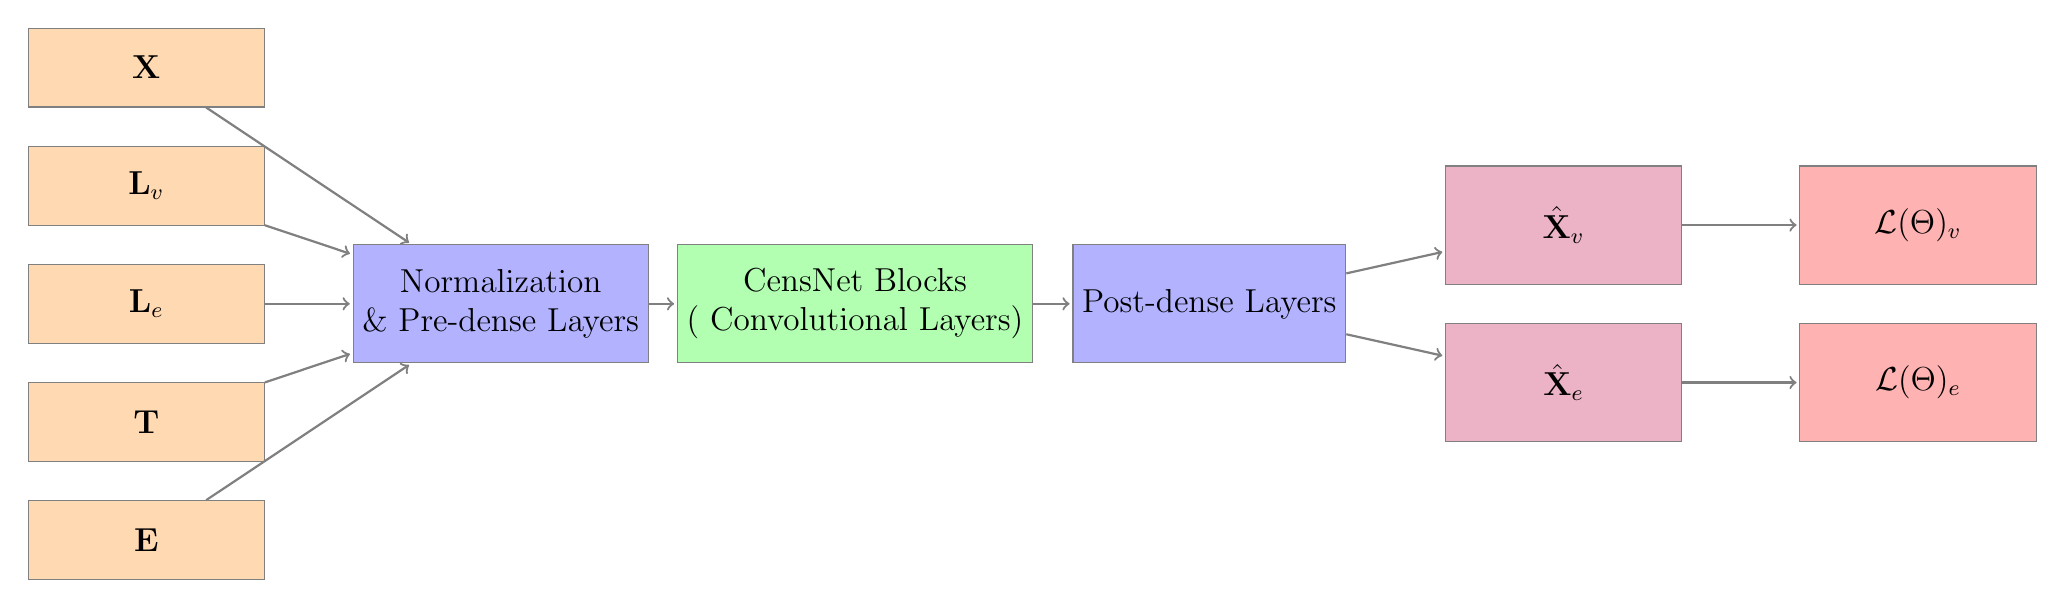
\begin{tikzpicture}[shorten >=1pt, ->, draw=black!50, node distance=1.5cm and 3.5cm, align=center]

    % Styles
    \tikzstyle{input} = [rectangle, draw, fill=orange!30, minimum width=3cm, minimum height=1cm, text centered, font=\large]
    \tikzstyle{dense} = [rectangle, draw, fill=blue!30, minimum width=3cm, minimum height=1.5cm, text centered, font=\large]
    \tikzstyle{conv} = [rectangle, draw, fill=green!30, minimum width=3cm, minimum height=1.5cm, text centered, font=\large]
    \tikzstyle{output} = [rectangle, draw, fill=purple!30, minimum width=3cm, minimum height=1.5cm, text centered, font=\large]
    \tikzstyle{loss} = [rectangle, draw, fill=red!30, minimum width=3cm, minimum height=1.5cm, text centered, font=\large]
    \tikzstyle{arrow} = [->, thick]

    % Input Layer
    \node[input] (node_features) at (0,0) {\(\mathbf{X}\)}; % Node Features
    \node[input] (node_laplacian) [below of=node_features] {\(\mathbf{L}_v\)}; % Node Laplacian
    \node[input] (edge_laplacian) [below of=node_laplacian] {\(\mathbf{L}_e\)}; % Edge Laplacian
    \node[input] (incidence_matrix) [below of=edge_laplacian] {\(\mathbf{T}\)}; % Incidence Matrix
    \node[input] (edge_features) [below of=incidence_matrix] {\(\mathbf{E}\)}; % Edge Features

    % Normalization and Pre-dense Layer
    \node[dense] (norm_pre_dense) [right of=edge_laplacian, xshift=3cm] {Normalization \\ \& Pre-dense Layers};

    % Convolutional Layers
    \node[conv] (conv_layers) [right of=norm_pre_dense, xshift=3cm] { CensNet Blocks \\ ( Convolutional Layers)};

    % Post-dense Layer
    \node[dense] (post_dense) [right of=conv_layers, xshift=3cm] {Post-dense Layers};

    % Outputs
    \node[output] (node_output) [right of=post_dense, xshift=3cm, yshift=1cm] {\(\hat{\mathbf{X}}_v\)}; % Node Predictions
    \node[output] (edge_output) [right of=post_dense, xshift=3cm, yshift=-1cm] {\(\hat{\mathbf{X}}_e\)}; % Edge Predictions

    % Losses
    \node[loss] (node_loss) [right of=node_output, xshift=3cm] {\(\mathcal{L}(\Theta)_v\)};
    \node[loss] (edge_loss) [right of=edge_output, xshift=3cm] {\(\mathcal{L}(\Theta)_e\)};

    % Arrows
    \draw[arrow] (node_features) -- (norm_pre_dense);
    \draw[arrow] (node_laplacian) -- (norm_pre_dense);
    \draw[arrow] (edge_laplacian) -- (norm_pre_dense);
    \draw[arrow] (incidence_matrix) -- (norm_pre_dense);
    \draw[arrow] (edge_features) -- (norm_pre_dense);

    \draw[arrow] (norm_pre_dense) -- (conv_layers);

    \draw[arrow] (conv_layers) -- (post_dense);

    \draw[arrow] (post_dense) -- (node_output);
    \draw[arrow] (post_dense) -- (edge_output);

    \draw[arrow] (node_output) -- (node_loss);
    \draw[arrow] (edge_output) -- (edge_loss);

\end{tikzpicture}

